\documentclass[12pt]{extarticle}
\usepackage{geometry}
\geometry{
a4paper,
total={170mm,257mm},
left=20mm,
top=20mm,
headheight=12pt
}

\usepackage[parfill]{parskip} % Activate to begin paragraphs with an empty line rather than an indent
\usepackage{amsmath}
\usepackage{amsfonts}
\usepackage{tikz,pgfplots}
\usepackage{gensymb}
\usepackage{graphicx}
\usepackage{subcaption}
\usepackage{xurl}


\usepackage{epstopdf}
%\usepackage{listings}
\usepackage{tikz,fp,fp-random,todonotes}
\usepackage[procnames]{listings}
\usepackage{afterpage}
\usepackage{float}
\usepackage{amsthm}
\usepackage{wrapfig}
\usepackage{booktabs,caption}
\usepackage[flushleft]{threeparttable}
\usepackage{scrextend}
\usepackage[all]{nowidow}
\usepackage{stfloats}
\usepackage{mathtools}
\usepackage{bm}
\usepackage{stackengine}
\usepackage[hidelinks]{hyperref}
\usepackage{siunitx}
%\usepackage{subfig}
\usepackage{authblk}
\usepackage{cleveref}

% less space before sections 
% \titlespacing*{<command>}{<left>}{<before-sep>}{<after-sep>}
\usepackage{titlesec}
\titlespacing*{\section}
{0pt}{2ex plus 1ex minus .2ex}{2ex plus .2ex}
\titlespacing*{\subsection}
{0pt}{1ex plus 1ex minus .2ex}{1ex plus .2ex}
\titlespacing*{\paragraph}
{0pt}{1ex plus 1ex minus .2ex}{1ex plus .2ex}
 
\addtokomafont{labelinglabel}{\sffamily}


\usetikzlibrary{calc}
\usetikzlibrary{backgrounds}
\usetikzlibrary{calc}
\usetikzlibrary{decorations.markings}
\usetikzlibrary{arrows}
\usetikzlibrary{positioning}
\usetikzlibrary{decorations.text}

\usetikzlibrary{shadings}
\usetikzlibrary{backgrounds}
\usetikzlibrary{calc}
\usetikzlibrary{decorations.markings}
\usetikzlibrary{arrows}
\usetikzlibrary{positioning}
\usetikzlibrary{decorations.text}
\usetikzlibrary{shapes.multipart}
        
\allowdisplaybreaks
\renewcommand{\floatpagefraction}{.85}

\newcommand{\x}{{\bf x}}
\renewcommand{\d}{{\rm d}}
\newcommand{\e}{{\rm e}}
\newcommand{\ii}{{\rm i}}

\newcommand{\tmi}{\tau_0\wedge\tau}
\newcommand{\tma}{\tau_0\vee\tau}
\newcommand{\taua}{\tau_{\rm A}}

% appendix
\usepackage[title,page]{appendix}
\usepackage{chngcntr}

% Supplementary
% https://support.authorea.com/en-us/article/how-to-create-an-appendix-section-or-supplementary-information-1g25i5a/
\newcommand{\beginsupplement}{%
      	\setcounter{table}{0}
        \renewcommand{\thetable}{S\arabic{table}}%
        \setcounter{figure}{0}
        \renewcommand{\thefigure}{S\arabic{figure}}%
		\setcounter{equation}{0}
        \renewcommand{\theequation}{A\arabic{equation}}%
}

% line numbers
\usepackage[displaymath, mathlines]{lineno}
\renewcommand\linenumberfont{\normalfont\small\sffamily}
%\linenumbers
\modulolinenumbers[2]

% Title page
\title{Modeling the effect of aneuploidy on cancer evolution}
% Authors
\renewcommand\Affilfont{\small}

\author[1]{Remus Stana}
\author[2]{Uri Ben-David}
\author[3]{Daniel B. Weissman}
\author[1,*]{Yoav Ram}
\affil[1]{School of Zoology, Faculty of Life Sciences, Tel Aviv University}
\affil[2]{Department of Human Molecular Genetics and Biochemistry, Faculty of Medicine, Tel Aviv University}
\affil[3]{Department of Physics, Emory University}
\affil[*]{Corresponding author: yoav@yoavram.com}
 
%%%%%%%%%%%%%%%%%%%%%%%%%%%%%%%%%%%%%%%%%%
\begin{document}
\maketitle

%%%%%%%%%%%%%%%%%%%%%%%%%%%%%%%%%%%%%%%%%%
\begin{abstract}
Evolutionary rescue is the process by which a population is able to survive a sudden environmental change which initially causes the population to decline towards extinction. A prime example of evolutionary rescue is the ability of cancer to survive being exposed to various treatments. We are interested in the mechanisms through which a population of cancer cells are able to adapt to chemotherapy, and in particular, the role played by chromosomal instability (aneuploidy). Cancer cells which have aneuploidy are hypothesized to have a higher fitness in an environment altered by anti-cancer drugs as they have incomplete pathways which drugs activate in order to kill the cells. Aneuploidy is highly prevalent in tumors and certain drugs which attempt to combat cancers through increasing chromosomal instability. As a result, the question we wish to answer is how aneuploidy impacts the fate of the population of cancer cells. We propose to model evolutionary rescue with the help of multi-type branching processes to obtain the probability that cancer will survive. Additionally, we will utilize large genomic datasets to asses the effects of aneuploidy on the probability of evolutionary rescue.
\end{abstract}

\newpage
%%%%%%%%%%%%%%%%%%%%%%%%%%%%%%%%%%%%%%
\section*{Introduction}

% TODO remove the commented out paragraphs if you dont need them. OK

%%%%%%

% OVERVIEW OF INTRODUCTION:
% - background on CIN in cancer
% - what hasn't been done? (aneuploidy + drug resistance)
% - why is that important?
% - how we tackle this background
% - summary of our analysis
% history of evolutionary rescue literature (that is not specific to cancer) should move to literature, and we should have a clear statement on what we add to that literature. 

\paragraph{Aneuploidy in cancer.} Chromosomal instability (CIN) is the mitotic process in which cells suffer from chromosome mis-segregation that leads to aneuploidy, where cells are characterized by structural changes of the chromosomes and copy number alterations \cite{schukken2018cin}.
Interestingly, aberrations in chromosome copy number have been shown to allow cancer cells to survive under stressful conditions such as drug therapy.
Indeed, cancer cells are often likely to be aneuploid, and aneuploidy is associated with poor patient outcomes \cite{ben2020context}.

% this belong in the next paragraph, or remove it altogether
% One mechanism by which aneuploidy has been hypothesized to affect cancer is by providing phenotypic variation and increasing heterogeneity in a tumor. 

The role of chromosomal instability (CIN) in the emergence of cancer has been studied extensively in the past decades \cite{michor2005can,christine2018understanding,nowak2002role,pavelka2010dr,komarova2003mutation,zhu2018cellular}.
One hypothesis is that CIN facilitates tumor genesis by accelerating the removal of tumor suppression genes (TSG) and subsequent appearance of cancer. The deletion of tumor suppression genes can happen in two ways: two point mutations deleting both alleles of the TSG (assuming a diploid genotype), or one point mutation and one chromosomal loss event.
Initial theoretical studies have shown that aneuploidy can have a significant role in the deletion of the the tumor suppressing genes when compared to two consecutive point mutations \cite{nowak2002role,komarova2003mutation,michor2005can,komarova2008selective}. % TODO mention if studies are theoretical , experimental, or clinical OK
However, when taking into account that the appearance of aneuploidy requires a mutation to trigger CIN, the probability that CIN precedes tumor genesis is highly unlikely.

\paragraph{Evolutionary rescue.} Populations adapted to a certain environment are vulnerable to environmental changes, which might cause extinction of the population. Examples of such environmental changes include climate change, invasive species or the onset of drug therapies. Adaptation is a race against time as the population size decreases in the new environment~\cite{tanaka2022surviving}. 
{\em Evolutionary rescue} is the process where the population acquires a trait that increases fitness in the new environment such that extinction is averted. It is mathematically equivalent to the problem of crossing of fitness valley \cite{weissman2009rate,weissman2010rate}.
There are three potential ways for a population to survive environmental change: migration to a new habitat similar to the one before the onset of environmental change \cite{cobbold2020should}; adaptation by phenotypic plasticity without genetic modification \cite{carja2019evolutionary,carja2017evolutionary,levien2021non}; and adaptation through genetic modifications, e.g., mutation \cite{uecker2014evolutionary,uecker2016role,uecker2011fixation}.

Models of evolutionary rescue usually assume that the fitness of the wildtype and mutant are independent of time. An exception is \cite{marrec2020adapt}, where the fitness of the wildtype and mutant are time dependent. Additionally, \cite{uecker2011fixation} investigated the probability of fixation of a beneficial mutation in a variable environment with arbitrary time-dependent selection coefficent and population size.
Most models focus on the probability that at least one mutation rescues the population. How multiple mutations contribute to the survival of the population is less explored. One exception is \cite{wilson2017soft} which showed that evolutionary rescue is significantly enhanced by soft selective sweeps when multiple mutations contribute. 
Evolutionary rescue that requires two successive mutations has been investigated by \cite{martin2013probability} with the help of diffusion approximation.


%%%%%%%%%%%%%%%%%%%%%%%%%%%%%%%%%%%%%%%%%%
\section*{Methods}
\subsection*{Evolutionary model}

We follow the number of cancer cells that belong to three different types at time $t$: wildtype euploid, $w_t$; wildtype aneuploid, $a_t$; and mutant euploid, $m_t$. 
These cells grow and die with rates $\lambda_k$ and $\mu_k$ for $k=w, a, m$.
Wildtype cells become aneuploid at rate $u$. Aneuploid and wildtype cells mutate with rate $v$ (Figure \ref{figureAneuploidy}). 
Thus, the changes in the number of each cell type is described by
\begin{subequations}
\begin{flalign}
w_t&\rightarrow w_t+1:\quad \lambda_ww_t,\\
w_t&\rightarrow w_t-1:\quad \left(\mu_w+u+v\right)w_t,\\
a_t&\rightarrow a_t+1:\quad \lambda_aa_t+uw_t,\\
a_t&\rightarrow a_t-1:\quad \left(\mu_a+v\right)a_t,\\
m_t&\rightarrow m_t+1:\quad \lambda_am_t+va_t+vm_t,\\
m_t&\rightarrow m_t-1:\quad \mu_am_t.
\end{flalign}
\end{subequations}

The difference between growth and death is $\Delta_k = \lambda_k-\mu_k$.
We assume that $\Delta_w<0$ due to drug therapy (or some other stress), and that $\Delta_m$ due to resistance conferred by the mutant.
We analyze two cases: in the first, aneuploid cells are partially resistant, $\Delta_m>\Delta_a>0$; in the second, aneuploid cells are tolerant, $0>\Delta_a>\Delta_w$  \cite{brauner2016distinguishing}.

Here, \emph{evolutionary rescue} occurs when the aneuploid cells are able to either prevent (when $\Delta_a>0$) or delay (when $0>\Delta_a>\Delta_w$) the extinction of the cancer-cell population before the adaptive mutant cells appear and fixate in the populaiton.
To analyze evolutionary rescue in this model, we use the framework of \emph{multitype branching processes} \cite{rybnikov2021fitness,harris1963theory}. 
This allows us to find explicit expressions for the survival probability of the population--the probability that it does not become extinct due to stressful conditions, e.g., drug therapy.
Note that branching processes imply that lineages produced by cells from the initial population grow and die independently of each other.
This is a necessary simplification, but it is unrealistic, as cells usually compete for resources.
A more realistic model may include competition on limited resources between lineages, as well as spatial structure, which may play an important role in the development of cancer \cite{martens2011spatial}.

The survival probability of a population consisting initially of one wildtype cell satisfies the quadratic equation,
\begin{equation} \label{quadraticeqev1}
\begin{aligned}
1-p_w = & \frac{\mu_w}{\lambda_w+\mu_w+u+v} + 
		  \frac{u}{\lambda_w+\mu_w+u+v}\left(1-p_a\right) + \\
		  & \frac{\lambda_w}{\lambda_w+\mu_w+u+v}\left(1-p_w\right)^2 +
		  \frac{v}{\lambda_w+\mu_w+u+v}\left(1-p_m\right) ,
\end{aligned}
\end{equation}
where the $p_w$, $p_a$, and $p_m$ are the survival probabilities of a population consisting initially of one wildtype cell, one aneuploid cell, and one mutant cell, respectively.

The smallest solution of the quadratic equation \cref{quadraticeqev1} gives the survival probability, which still depends on both $p_a$ and $p_m$,
\begin{align}\label{survprobw}
p_w=\frac{\lambda_w-\mu_w-u-v+\sqrt{\left(\lambda_w-\mu_w-u-v\right)^2+4\lambda_w\left(up_a+vp_m\right)}}{2\lambda_w} .
\end{align}

If the population originally consists of a single aneuploid cell, then the probability that the population will survive is given by the quadratic equation
\begin{align}
1-p_a=\frac{\mu_a}{\lambda_a+\mu_a+v}+\frac{v}{\lambda_a+\mu_a+v}\left(1-p_m\right)+\frac{\lambda_a}{\lambda_a+\mu_a+v}\left(1-p_a\right)^2,
\end{align}
whose smallest solution is the survival probability:
\begin{align}\label{survproba}
p_a=\frac{\lambda_a-\mu_a-v+\sqrt{\left(\lambda_a-\mu_a-v\right)^2+4\lambda_avp_m}}{2\lambda_a}.
\end{align}

The probability that a single mutant cell survives is given by (Appendix \ref{AppendixSurvLin}):
\begin{equation}
p_m = \left\{
  \begin{array}{@{}ll@{}}
  \frac{\lambda_m-\mu_m}{\lambda_m},\quad \text{if }\lambda_m>\mu_m \\
   0,\quad \text{else} .
  \end{array}\right .
\end{equation}

% TODO add subsection on the Gillespie simulations OK
\subsection*{Evolutionary simulation} 
Simulations are performed using a \emph{Gillespie algorithm} \cite{gillespie1976general,gillespie1977exact} implemented in Python \cite{python}.
The simulation monitors the number of cells of each type: wildtype, aneuploid, and mutant. 
The wildtype population initially consists of $w_0$ cells, whereas the other cell types are initially absent.


At each iteration of the simulation loop we compute the rate $\nu_j$ of each event $j$. % TODO explains what events can occur and how you compute their rates, refer to illustration figure  OK
The sate of the stochastic system at time $t$ is represented by the triplet $\left(w_t,a_t,m_t\right)$ which can change in the time interval $\Delta_t$ according to the following events with appropriate rates (see Figure \ref{figureAneuploidy}):
\begin{subequations}
\begin{flalign*}
(+1,0,0)&:\quad \lambda_ww_t\quad\left(\text{birth euploid cell}\right),\\
(-1,0,0)&:\quad \mu_ww_t\quad\left(\text{death euploid cell}\right),\\
(-1,+1,0)&:\quad uw_t\quad\left(\text{euploid cell aquires aneuploidy}\right),\\
(-1,0,+1)&:\quad vw_t\quad\left(\text{euploid cell aquires mutation}\right),\\
(0,+1,0)&:\quad \lambda_aa_t\quad\left(\text{birth aneuploid cell}\right),\\
(0,-1,0)&:\quad \mu_aa_t\quad\left(\text{death aneuploid cell}\right),\\
(0,-1,+1)&:\quad va_t\quad\left(\text{aneuploid cell aquires mutation}\right),\\
(0,0,+1)&:\quad \lambda_am_t\quad\left(\text{birth mutant cell}\right),\\
(0,0,-1)&:\quad \mu_am_t\quad\left(\text{death mutant cell}\right).
\end{flalign*}
\end{subequations}
We then draw the time until the next event, $\Delta t$, from an exponential distribution whose rate parameter is the sum of the rates of all events, such that $\Delta t \sim \textit{Exp}(\sum_j \nu_j)$.
Then, we randomly determine which event occurred, where the probability for event $j$ is $p_j=\nu_j/\sum_i \nu_i$.
Finally, we update the number of cells of each type according to the event that occurred and update the time from $t$ to $t+\Delta t$. % TODO more details - you need to specify the events and how they change the number of cells. OK
We repeat these iterations until either the population becomes extinct (the number of cells of all types is zero) or the number of mutant cells is high enough so that its extinction probability is $<1\%$. % TODO how do you determine the extinction prob? ref to equation OK
We continue running the simulation until:
\begin{equation*}
m_t>\left\lfloor-\frac{3\log10}{\log\left(\frac{\mu_m}{\lambda_m}\right)}\right\rfloor+1,
\end{equation*}
which is the population size at which the extinction probability of the population of mutant cell is less then $1\%$. 
% TODO do you use tau leap? if so, update the text accordingly. OK
When the size of the initial population is large we utilize $\tau$-leaping where the increment of population change in a fixed time interval $\Delta t$ is Poisson distributed with mean $\nu_i\Delta t$ for each population $i$ \cite{gillespie2001approximate}. If the increment is negative and larger then the subpopulation size then updated 
\paragraph{Data availability.} All source code is available online at \url{https://github.com/yoavram-lab/EvolutionaryRescue}.

%%%%%%%%%%%%%%%%%%%%%%%%%%%%%%%%%%%%%%%%%%
% TODO combine all diagram figures to a single figure with multiple panels. and make it fit in a single page. OK

%%%%%%

\begin{figure}
\centering
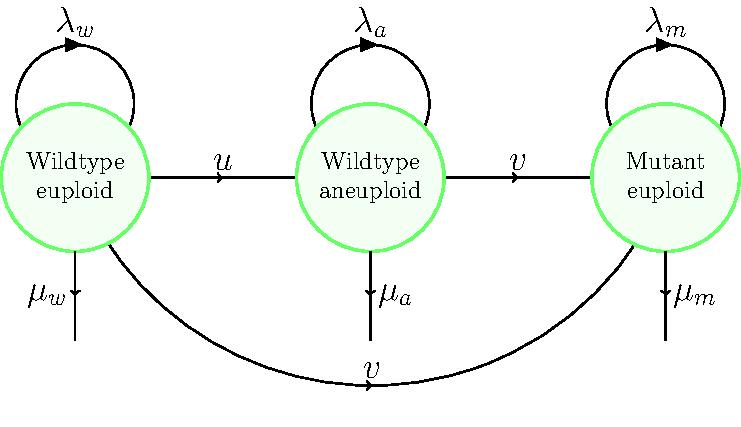
\includegraphics[width=0.55\textwidth]{Figures/figureAneuploidy3.pdf}
%\caption{}

%\end{subfigure}

\caption{\textbf{Model illustration.}
A population of cancer cells is subdivided to wildtype euploid, wildtype aneuploid and mutant euploid cells, which divide with rates $\lambda_w$, $\lambda_a$, and $\lambda_m$, respectively, and die at rates $\mu_w$, $\mu_a$, and $\mu_m$, respectively. 
Wildtype cells can become aneuploid at rate $u$. Both aneuploid and wildtype cells can acquire a beneficial mutation with rate $v$.}
\label{figureAneuploidy}
\end{figure}

%%%%%%%%%%%%%%%%%%%%%%%%%%%%%%%%%%%%%%%%%%%%%%%%%%%%%%%%

%\newpage
\section*{Results}

% OVERVIEW OF RESULTS 

%%%%%%%%%%%%%%%%%%%%%%%%%%%%%%%%%%%%%%%%%%%%%%%%%%%%%%%%
% TODO give a descriptive name instead of a mathematical formula OK
%\subsection*{First case: $4\lambda_avp_m<\left(\lambda_a-\mu_a-v\right)^2$}
\subsection*{First case: Highly deleterious or highly beneficial aneuploidy}

\paragraph{Aneuploid cells are drug resistant.} 
We first assume wildtype cells are susceptible to the drug, $\lambda_w<\mu_w$, whereas aneuploid cells are resistant, $\lambda_a>\mu_a$.
Thus, we rewrite \cref{survprobw,survproba} as
\begin{align*}
p_a&=\frac{\lambda_a-\mu_a-v}{2\lambda_a}\left(1+\sqrt{1+\frac{4\lambda_avp_m}{\left(\lambda_a-\mu_a-v\right)^2}}\right),\\
p_w&=\frac{\lambda_w-\mu_w-u-v}{2\lambda_w}\left(1-\sqrt{1+\frac{4\lambda_w\left(vp_m+up_a\right)}{\left(\lambda_w-\mu_w-u-v\right)^2}}\right).
\end{align*}
Using a quadratic Taylor expansion, $\sqrt{1+x}=1+x/2+O(x^2)$, 
we obtain the following approximation for the survival probability of a population consisting of a single individual wildtype cell (assuming $u,v \ll 1$),
\begin{align}\label{survprobwinitial}
p_w 
&\approx -\frac{vp_m+up_a}{\lambda_w-\mu_w-u-v}\\
\nonumber
%&\approx-\frac{1}{\lambda_w-\mu_w-u-v}\left[\frac{v\left(\lambda_a-\mu_a-u\right)}{\lambda_a}+\frac{uv\left(\lambda_m-\mu_m\right)}{\lambda_m\left(\lambda_a-\mu_a-u\right)}+\frac{v\left(\lambda_m-\mu_m\right)}{\lambda_m}\right]\\ \label{survprobw2}
&\approx-\frac{1}{\lambda_w-\mu_w}\left[\frac{v\left(\lambda_a-\mu_a\right)}{\lambda_a}+\frac{uv\left(\lambda_m-\mu_m\right)}{\lambda_m\left(\lambda_a-\mu_a\right)}+\frac{v\left(\lambda_m-\mu_m\right)}{\lambda_m}\right].
\end{align}

We write \cref{survprobw} as
\begin{equation}\label{survprobwapprox1}
p_w=-\frac{1}{\Delta_w}\left(\frac{v\Delta_a}{\lambda_a}+\frac{uv\Delta_m}{\lambda_m\Delta_a}+\frac{v\Delta_m}{\lambda_m}\right).
\end{equation}
So, given an initial population of $N$ wildtype cells, the probability that the population will survive is given by
\begin{align}\label{aneuploidyresistentfirstapprox}
p_{est}=1-\left(1-p_w\right)^N\approx 1-\e^{-Np_w}=1-\exp\left[\frac{N}{\Delta_w}\left(\frac{v\Delta_a}{\lambda_a}+\frac{uv\Delta_m}{\lambda_m\Delta_a}+\frac{v\Delta_m}{\lambda_m}\right)\right] .
\end{align}
\Cref{SurvPlot} shows that the survival probability, $p_{est}$, quickly grows as the wildtype growth rate, $\lambda_w$, increases. % Todo I dont think this figure should show lambda_w>1, as in that case the wildtype is resistant and there is no rescue scenario. OK
\Cref{SurvPlotNData} show $p_{est}$ as a function of $N$, including comparison of our approximation \eqref{aneuploidyresistentfirstapprox} % ref to equation OK
and simulation results.

%%%%%%%%%%%%%%%%%%%%%%%%%%%%%%%%%%%%%%%%%%
\begin{figure}[!t]
 \vspace*{1\baselineskip}
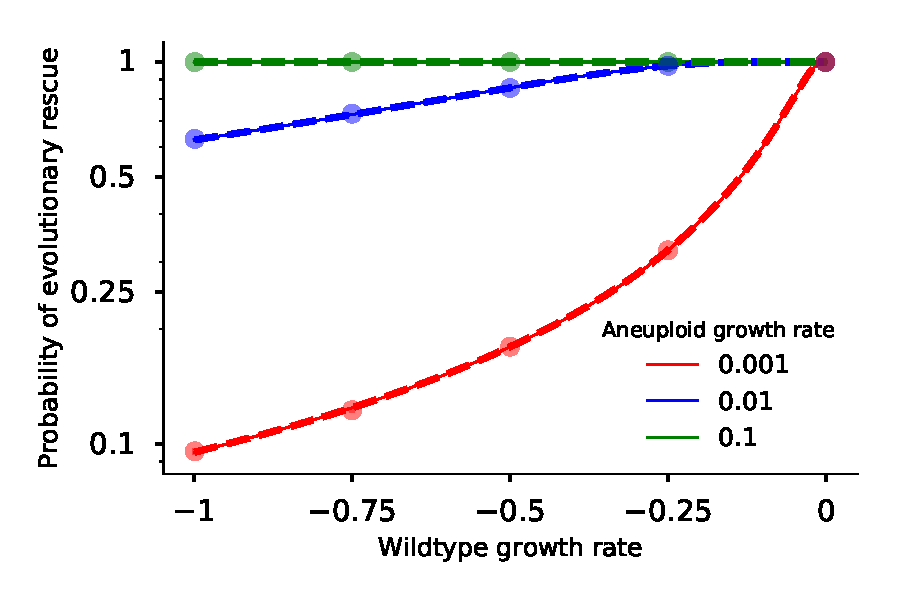
\includegraphics[width=1\textwidth]{Figures/P_est_growth.pdf}
\caption{Plot of the probability of survival of a population as a function of the proliferation rate of the wildtype cells. The continuous lines represent the exact result \eqref{survprobw} while the dashed lines represent the approximation \eqref{survprobwapprox1}. Here the population initially consists of $N$ wildtype cells and for the simulations we have chosen the following parameters: $N=10^4, \lambda_a=1+10^{-2},\lambda_m=1+10^{-1},\mu_w=1,\mu_a=1,\mu_m=1$. The error bars represent $95\%$ confidence interval of the form $p\pm1.96\sqrt{p\left(1-p\right)/n}$ where $p$ is the mean probability of evolutionary rescue and $n$ is the number of simulations. The error bars are present but are not visible given the fact that we have used $10^5$ simulations for each combination of parameters.}
\label{SurvPlot}
\end{figure}
%%%%%%%%%%%%%%%%%%%%%%%%%%%%%%%%%%%%%%%%%%

We want to improve the accuracy of our approximation by taking into consideration the second term of the Taylor series expansion:
\begin{align*}
\left(1+\frac{4\lambda_avp_m}{\left(\lambda_a-\mu_a-v\right)^2}\right)^{\frac{1}{2}}=1+\frac{2\lambda_avp_m}{\left(\lambda_a-\mu_a-v\right)^2}-\frac{\left(\lambda_avp_m\right)^2}{4\left(\lambda_a-\mu_a-v\right)^4}+\cdots,
\end{align*}
which gives us the following approximation for $p_a$:
\begin{align}
p_a=\frac{\lambda_a-\mu_a-v}{\lambda_a}+\frac{vp_m}{\lambda_a-\mu_a-v}-\frac{\lambda_a\left(vp_m\right)^2}{8\left(\lambda_a-\mu_a-v\right)^3}
\end{align}
From which we deduce that:
\begin{align}\nonumber
p_w&\approx-\frac{1}{\lambda_w-\mu_w-u-v}\left[\frac{v\left(\lambda_a-\mu_a-u\right)}{\lambda_a}+\frac{uv\left(\lambda_m-\mu_m\right)}{\lambda_m\left(\lambda_a-\mu_a-u\right)}+\frac{v\left(\lambda_m-\mu_m\right)}{\lambda_m}-\frac{uv^2\lambda_a\left(\lambda_m-\mu_m\right)^2}{8\lambda_m^2\left(\lambda_a-\mu_a-v\right)^3}\right]\\ \label{survprobw3}
&\approx-\frac{1}{\lambda_w-\mu_w}\left[\frac{v\left(\lambda_a-\mu_a\right)}{\lambda_a}+\frac{uv\left(\lambda_m-\mu_m\right)}{\lambda_m\left(\lambda_a-\mu_a\right)}+\frac{v\left(\lambda_m-\mu_m\right)}{\lambda_m}-\frac{uv^2\lambda_a\left(\lambda_m-\mu_m\right)^2}{8\lambda_m^2\left(\lambda_a-\mu_a\right)^3}\right].
\end{align}
Using the notations described in \eqref{notationalconv} we write the above equation as:
\begin{equation}\label{survprobwapproxcorrected}
p_w=-\frac{1}{\Delta_w}\left(\frac{v\Delta_a}{\lambda_a}+\frac{uv\Delta_m}{\lambda_m\Delta_a}+\frac{v\Delta_m}{\lambda_m}-\frac{uv^2\lambda_a\Delta_m^2}{8\lambda_m^2\Delta_a^3}\right).
\end{equation}
Given an initial population consisting of $N$ wildtype cancer cells, the probability that the population will survive is given by: 
\begin{align}
p_{est}=1-\left(1-p_w\right)^N\approx 1-\e^{-Np_w}=1-\exp\left[\frac{N}{\Delta_w}\left(\frac{v\Delta_a}{\lambda_a}+\frac{uv\Delta_m}{\lambda_m\Delta_a}+\frac{v\Delta_m}{\lambda_m}-\frac{uv^2\lambda_a\Delta_m^2}{8\lambda_m^2\Delta_a^3}\right)\right].
\end{align}


\paragraph{$\lambda_a<\mu_a$ and $\lambda_w<\mu_w$.}
We assume that $\lambda_a<\mu_a$ and $\lambda_w<\mu_w$ and, as a result, we rewrite \eqref{survprobw} and \eqref{survproba} as:
\begin{align*}
p_a&=\frac{\lambda_a-\mu_a-v}{2\lambda_a}\left(1-\sqrt{1+\frac{4\lambda_avp_m}{\left(\lambda_a-\mu_a-v\right)^2}}\right),\\
p_w&=\frac{\lambda_w-\mu_w-u-v}{2\lambda_w}\left(1-\sqrt{1+\frac{4\lambda_w\left(vp_m+up_a\right)}{\left(\lambda_w-\mu_w-u-v\right)^2}}\right).
\end{align*}
\begin{align}\label{survprobwinitial}
p_w&\approx-\frac{vp_m+up_a}{\lambda_w-\mu_w-u-v}\\
\nonumber
&\approx\frac{1}{\lambda_w-\mu_w-u-v}\left[\frac{uv\left(\lambda_m-\mu_m\right)}{\lambda_m\left(\lambda_a-\mu_a-v\right)}-\frac{v\left(\lambda_m-\mu_m\right)}{\lambda_m}\right]\\ \label{survprobw2}
&\approx\frac{v\left(\lambda_m-\mu_m\right)}{\lambda_m\left(\lambda_w-\mu_w\right)}\left[\frac{u}{\left(\lambda_a-\mu_a\right)}-1\right],
\end{align}
where in the last line we have used the fact that $u,v\ll1$. Using the notational convention
\begin{equation}\label{notationalconv}
\Delta_i=\lambda_i-\mu_i,
\end{equation}
we write \eqref{survprobw} as
\begin{equation}\label{survprobwapprox2}
p_w=\frac{v\Delta_m}{\lambda_m\Delta_w}\left(\frac{u}{\Delta_a}-1\right).
\end{equation}
Given an initial population consisting of $N$ wildtype cancer cells, the probability that the population will survive is given by: 
\begin{align}\label{AneuploidyDeleteriousApprox}
p_{est}=1-\left(1-p_w\right)^N\approx 1-\e^{-Np_w}=1-\exp\left[\frac{v\Delta_mN}{\lambda_m\Delta_w}\left(1-\frac{u}{\Delta_a}\right)\right],
\end{align}

%%%%%%%%%%%%%%%%%%%%%%%%%%%%%%%%%%%%%%%%%%
\begin{figure}[!t]
 \vspace*{1\baselineskip}
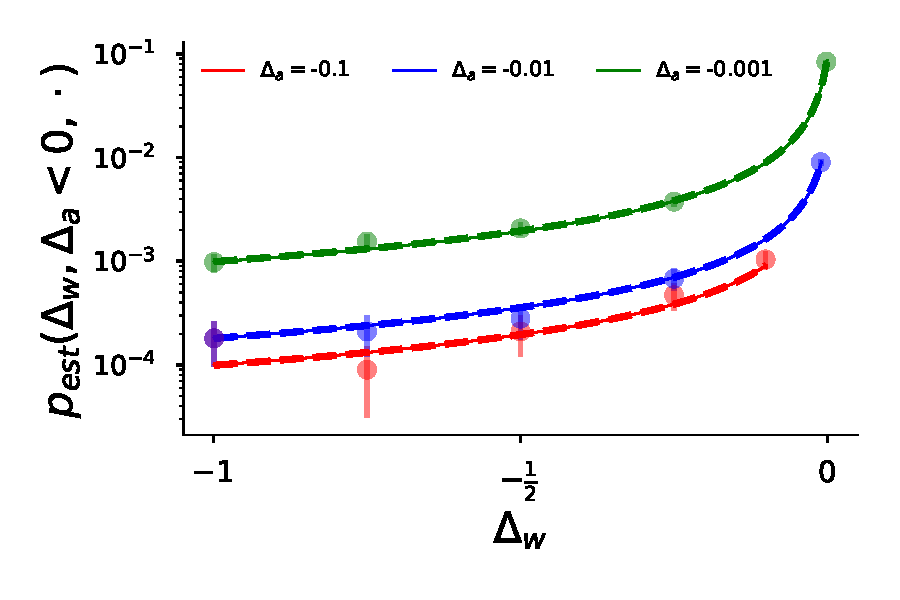
\includegraphics[width=1\textwidth]{Figures/P_est.pdf}
\caption{Plot of the survival probability of an initial population consisting of $10^{4}$ wildtype cells as a function of $\Delta_a=\lambda_a-\mu_a$ for various values of $\Delta_w=\lambda_a-\mu_a$. The continuous lines represent the exact result \eqref{survprobw} while the dashed lines represent the approximation \eqref{AneuploidyDeleteriousApprox}. The error bars represent $95\%$ confidence interval of the form $p\pm1.96\sqrt{p\left(1-p\right)/n}$ where $p$ is the mean probability of evolutionary rescue and $n$ is the number of simulations.}
\label{P_est}
\end{figure}

%%%%%%%%%%%%%%%%%%%%%%%%%%%%%%%%%%%%%%%%%%%%%%%%%%%%%%%%%%%%%%%%%%%%
\begin{figure}[!t]
 \vspace*{1\baselineskip}
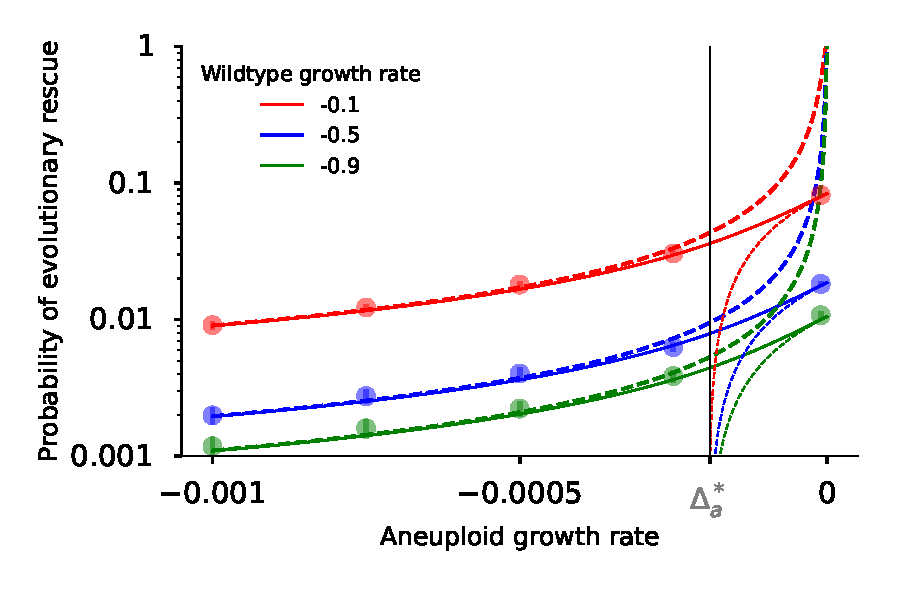
\includegraphics[width=1\textwidth]{Figures/P_est_divergence.pdf}
\caption{Plot of the survival probability of an initial population consisting of $10^{4}$ wildtype cells as a function of $\Delta_w=\lambda_w-\mu_w$ for various values of $\Delta_a=\lambda_a-\mu_a$. The continuous lines represent the exact result \eqref{survprobw} while the dashed lines represent the approximations \eqref{AneuploidyDeleteriousApprox}. The error bars represent $95\%$ confidence interval of the form $p\pm1.96\sqrt{p\left(1-p\right)/n}$ where $p$ is the mean probability of evolutionary rescue and $n$ is the number of simulations. The value highlighted in grey is the threshold $\Delta_a^*$ from \eqref{thresholdvalueaneuploid} which marks the transition between the regime dictated by \eqref{AneuploidyDeleteriousApprox} to the one dictated by \eqref{pestthirdcase}. }
\label{P_est}
\end{figure}

%%%%%%%%%%%%%%%%%%%%%%%%%%%%%%%%%%%%%%%%%%%%%%%%%%%%%%%%%%%%%%%%%%%%
\begin{figure}[!t]
 \vspace*{1\baselineskip}
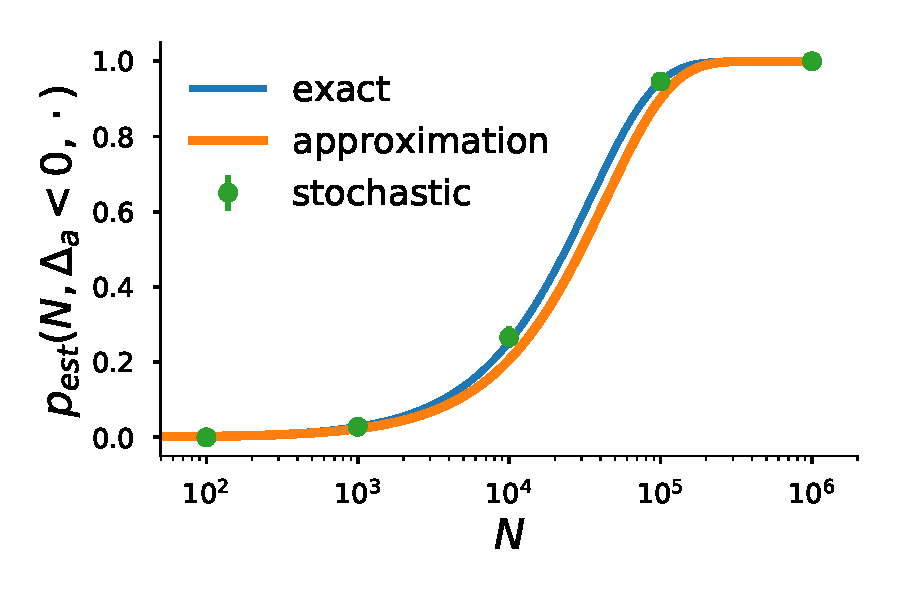
\includegraphics[width=1\textwidth]{Figures/DeleteriousTauLeapPlot.pdf}
\caption{Plot of the probability of survival of a population as a function of the initial population size of wildtype cells. The continuous lines represent the exact result \eqref{survprobw} while the dashed lines represent the approximation \eqref{pestthirdcase}. The error bars represent $95\%$ confidence interval of the form $p\pm1.96\sqrt{p\left(1-p\right)/n}$ where $p$ is the mean probability of evolutionary rescue and $n$ is the number of simulations. The error bars are present but are not visible given the fact that we have used $n=10^5$ simulations for each combination of parameters.}
\label{DeleteriousPlot}
\end{figure}

%%%%%%%%%%%%%%%%%%%%%%%%%%%%%%%%%%%%%%%%%%%%%%%%%%%%%%%%%%%%%%%%%%%%
%\subsection*{Second case: $4\lambda_avp_m>\left(\lambda_a-\mu_a-v\right)^2$}
\subsection*{Second case: Neutral aneuploidy}
If we assume that  $4\lambda_avp_m>\left(\lambda_a-\mu_a-v\right)^2$ then we write:
\begin{equation}
p_a=\frac{\lambda_a-\mu_a-v+2\sqrt{\lambda_a vp_m}\left(1+\frac{\left(\lambda_a-\mu_a-v\right)^2}{4\lambda_avp_m}\right)^{\frac12}}{2\lambda_a}
\end{equation}
and using the following Taylor series expansion:
\begin{align*}
\left(1+\frac{\left(\lambda_a-\mu_a-v\right)^2}{4\lambda_avp_m}\right)^{\frac{1}{2}}=1+\frac{\left(\lambda_a-\mu_a-v\right)^2}{8\lambda_avp_m}+\cdots
\end{align*}
we obtain:
\begin{align*}
p_a&\approx\frac{\lambda_a-\mu_a-v+2\sqrt{\lambda_a vp_m}\left[1+\frac{\left(\lambda_a-\mu_a-v\right)^2}{8\lambda_avp_m}\right]}{2\lambda_a}\\
&=\frac{\lambda_a-\mu_a-v+2\sqrt{\lambda_a vp_m}+\frac{\left(\lambda_a-\mu_a-v\right)^2}{4\sqrt{\lambda_avp_m}}}{2\lambda_a}\\
&=\frac{\left(\lambda_a-\mu_a-v+2\sqrt{\lambda_avp_m}\right)^2+4\lambda_avp_m}{8\lambda_a\sqrt{\lambda_avp_m}}\\
&=\frac{4\lambda_avp_m+4\lambda_avp_m\left(1+\frac{\lambda_a-\mu_a-v}{2\sqrt{\lambda_avp_m}}\right)^2}{8\lambda_a\sqrt{\lambda_avp_m}}\\
&=\frac{1}{2\lambda_a}\left(\lambda_a-\mu_a-v+2\sqrt{\lambda_avp_m}\right)
\end{align*}
As a result, we have from \eqref{survprobwinitial} the probability of rescue of a population starting from one wildtype individual:
\begin{align*}
p_w&\approx-\frac{1}{\lambda_w-\mu_w-u-v}\left[v\frac{\lambda_m-\mu_m}{\lambda_m}+\frac{u}{2\lambda_a}\left(\lambda_a-\mu_a-v+2\sqrt{\lambda_avp_m}\right)\right]\\
&=-\frac{1}{\lambda_w-\mu_w-u-v}\left[v\frac{\lambda_m-\mu_m}{\lambda_m}+\frac{u}{2\lambda_a}\left(\lambda_a-\mu_a-v\right)+u\sqrt{\frac{v\left(\lambda_m-\mu_m\right)}{\lambda_a\lambda_m}}\right]\\
&=-\frac{1}{\Delta_w-u-v}\left[v\frac{\Delta_m}{\lambda_m}+\frac{u\left(\Delta_a-v\right)}{2\lambda_a}+u\sqrt{\frac{v\Delta_m}{\lambda_a\lambda_m}}\right],
\end{align*}
where in the last line we have used the notations defined in \eqref{notationalconv}.

Given an initial population consisting of $N$ wildtype cancer cells, the probability that the population will survive is given by: 
\begin{align}\label{pestthirdcase}
p_{est}=1-\left(1-p_w\right)^N\approx 1-\e^{-Np_w}=1-\exp\left[\frac{N}{\Delta_w-u-v}\left(v\frac{\Delta_m}{\lambda_m}+\frac{u\left(\Delta_a-v\right)}{2\lambda_a}+u\sqrt{\frac{v\Delta_m}{\lambda_a\lambda_m}}\right)\right],
\end{align}
which we plot in Figure \ref{DeleteriousPlot} where we compare with numerical simulations and the exact result \eqref{survprobw}. The transition between the regimes defined by \eqref{AneuploidyDeleteriousApprox} and \eqref{pestthirdcase} respectively occurs at:
\begin{align}\label{thresholdvalueaneuploid}
\Delta_a^*=2vp_m+v+2\sqrt{vp_m\left(vp_m+\mu_a+v\right)}.
\end{align}

The probability of evolutionary rescue is given by:
\begin{equation}
p_{est}\sim\left\{
  \begin{array}{@{}ll@{}}
  1-\exp\left[\frac{N}{\Delta_w-u-v}\left(v\frac{\Delta_m}{\lambda_m}+\frac{u\left(\Delta_a-v\right)}{2\lambda_a}+u\sqrt{\frac{v\Delta_m}{\lambda_a\lambda_m}}\right)\right],\quad\text{if }4\lambda_avp_m>\left(\Delta_a-v\right)^2,\\
   1-\exp\left[\frac{v\Delta_mN}{\lambda_m\Delta_w}\left(1-\frac{u}{\Delta_a}\right)\right],\quad\text{if }\Delta_a<0\quad\text{and}\quad4\lambda_avp_m<\left(\Delta_a-v\right)^2,\\
   1-\exp\left[\frac{N}{\Delta_w}\left(\frac{v\Delta_a}{\lambda_a}+\frac{uv\Delta_m}{\lambda_m\Delta_a}+\frac{v\Delta_m}{\lambda_m}\right)\right],\quad\text{if }\Delta_a>0\quad\text{and}\quad4\lambda_avp_m<\left(\Delta_a-v\right)^2.
  \end{array}\right.
\end{equation}

%%%%%%%%%%%%%%%%%%%%%%%%%%%%%%%%%%%%%%%%%%%%%%%%%%%%%%%%%%%%
% TODO : should this move to methods? we only use this for simulations, right? should be in the Gillespie section?
\subsection*{Logistic growth}
We want to have birth and death rates which depends on the population size of wildtype $w$, aneuploidy $a$ and mutant $m$ cells:
\begin{align*}
&\lambda_w'=\lambda_w,\quad\mu_w'=\mu_w\\
&\lambda_a'=C_1+\left(\lambda_a-\mu_a\right)\left(1-\frac{w+a+m}{K}\right),\quad \mu_a'=C_1\\
&\lambda_m'=C_2+\left(\lambda_m-\mu_m\right)\left(1-\frac{w+a+m}{K}\right),\quad \mu_m'=C_2
\end{align*}
where $C_1, C_2>0$ are constants. We perform stochastic simulations for different values of the carrying capacity $K$ and we plot the results in Figure \ref{SurvPlotNDataLogisticKComplete}.  We observe that as $K$ increases the simulations converge to the analytic result which is because the carrying capacity is much larger then the population size of aneuploid cells for which the probability that the population is rescued is certain.

\begin{figure}[!t]
 \vspace*{1\baselineskip}
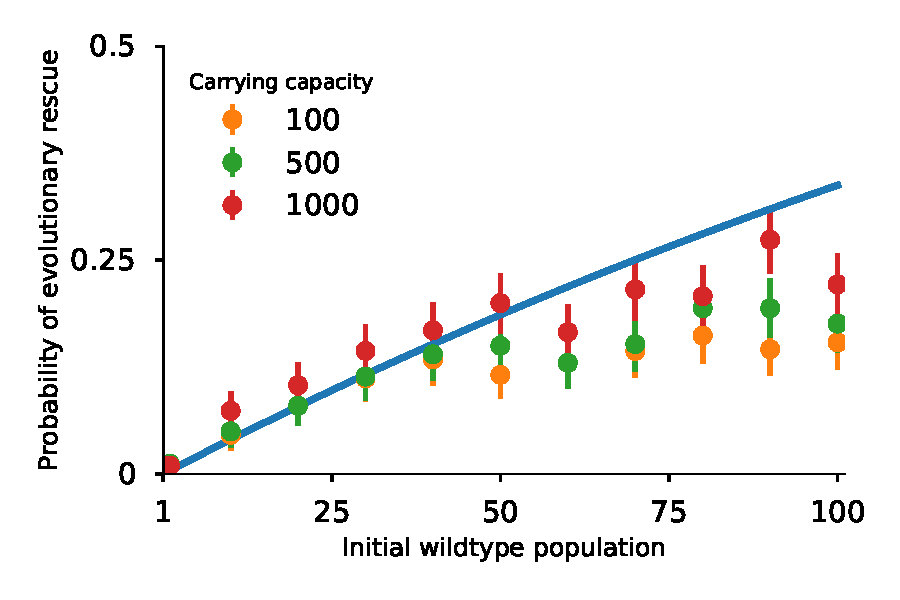
\includegraphics[width=1\textwidth]{Figures/SurvPlotNDataLogisticKComplete.pdf}
\caption{Plot of the survival probability of an initial population consisting of wildtype cells as a function of the initial population size.  Here the population initially consists of $N$ wildtype cells and for the simulations we have chosen the following parameters: $\lambda_w=1-10^{-1},\lambda_w=1+10^{-4},\lambda_m=1+10^{-1},\mu_w=1,\mu_m=1,u=10^{-2},v=10^{-7}, C_1=C_2=1$.}
\label{SurvPlotNDataLogisticKComplete}
\end{figure}


%%%%%%%%%%%%%%%%%%%%%%%%%%%%%%%%%%%%%%%%%%%%%%%%%%%%%%%%%%%%
\subsection*{Standing genetic variation}
So far we have assumed that the initial population of cells consisted entirely of wildtype cells.
We now modify this assumption so that the initial population includes a fraction $f$ of cells with aneuploidy.
The probability of evolutionary rescue by cells with aneuploidy from the initial population is
\begin{equation*}
p_{old} = 1-\left(1-p_a\right)^{fN}\approx 1-\e^{-fNp_a}.
\end{equation*}
The total probability of evolutionary rescue is given by
\begin{align}\nonumber
p_{total} 	&= p_{new}+\left(1-p_{new}\right)p_{old}\\
			&= 1-\exp\left(-\left[\left(1-f\right)p_w + fp_a\right]N\right) .
\end{align}

The fraction of cases in which the population is rescued by the standing genetic variation is given by $F\left(f\right)=\frac{p_{old}}{p_{total}}$.
%=\frac{ 1-\e^{-fNp_a}}{1-\e^{-\left[\left(1-f\right)p_w+fp_a\right]N}}.
Setting $F=\frac{1}{2}$, we use the expansion $\e^x \approx 1+x$ to obtain
\begin{equation}\label{halfeqstandvar}
f^*\approx\frac{p_w}{p_w+p_a},
\end{equation}
See \Cref{FractionPlot} for a demonstration of $F$ and $f*$.

%%%%%%%%%%%%%%%%%%%%%%%%%%%%%%%%%%%%%%%%%%
\subsection*{Rescue time}
%%%
\begin{figure}[!t]
 \vspace*{1\baselineskip}
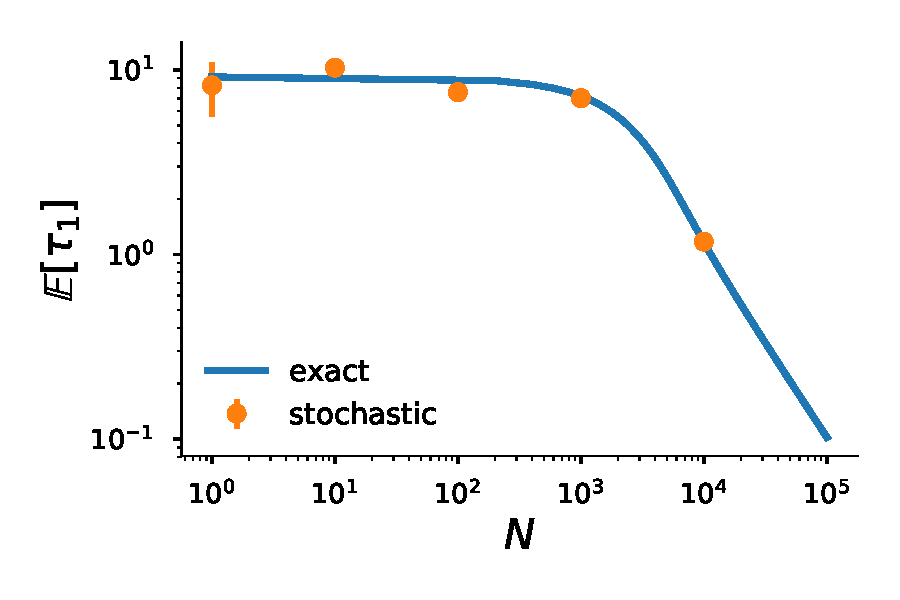
\includegraphics[width=1\textwidth]{Figures/MeanTimeGrowthAneuploidyPlot.pdf}
\caption{Plot of the mean time until the appearence of a resistence mutation which rescues the population in the case when evolutionary rescue is possible only through mutation but not aneuploidy and mutation.  Here the population initially consists of $N$ wildtype cells and for the simulations we have chosen the following parameters: $\lambda_w=1-10^{-1},\lambda_m=1+10^{-1},\mu_w=1,\mu_m=1,u=10^{-2},v=10^{-7}$.}
\label{MeanTimeGrowthAneuploidyPlot}
\end{figure}
We calculate the mean time for the appearance of the first mutant that rescues the cancer cell population.
Let $\tau=\tau_1+\tau_2$ be the time the first mutant cell that appears and rescues the population, where $\tau_1$ is the time at which the first aneuploid cell appears whose lineage will rescue the population and $\tau_2$ the time for this aneuploidy lineage to produce the first mutant that rescues the population. 
% something is missing in the next line...?
% the entire section is missing text...

The time $\tau_1$ can be aproximated by a inhomogeneus Poisson process:
\begin{align}
\tau_1\sim \text{Poisson}\left(\frac{1}{up_aw_t}\right),
\end{align}
where $w_t$ is the size of the wildtype population at time $t$: 
\begin{equation}
w_t=W_0\e^{\Delta_wt}.
\end{equation}
As a result, the probability density function of $\tau_1$ is given by:
\begin{align}
f\left(\tau_1\right)=R\left(\tau_1\right)\e^{-\int_0^{\tau_1} R(t)\d t}
\end{align}
We are interested in the time to appearence of the first succesful aneuploid cell conditional on population surving we have the following:
\begin{align*}
P\left(\tau_1<t\right)&=P\left(\tau_1<t|M\left(t\rightarrow\infty\right)\neq0\right)P\left(M\left(t\rightarrow\infty\right)\neq0\right)\\
&+P\left(\tau_1<t|M\left(t\rightarrow\infty\right)=0\right)P\left(M\left(t\rightarrow\infty\right)=0\right)\\
P\left(\tau_1<t\right)&=P\left(\tau_1<t|M\left(t\rightarrow\infty\right)\neq0\right)P\left(M\left(t\rightarrow\infty\right)\neq0\right)
\end{align*}
where we used the fact that evolutionary rescue is impossible when the mutant population is destined to be zero:
\begin{align*}
P\left(\tau_1<t|M\left(t\rightarrow\infty\right)=0\right)=0.
\end{align*}
As a result, we obtain 
\begin{align}
P\left(\tau_1<t|M\left(t\rightarrow\infty\right)\neq0\right)=\frac{P\left(\tau_1<t\right)}{1-\left(1-p_w\right)^N}
\end{align}
where we have used
\begin{equation}
P\left(M\left(t\rightarrow\infty\right)\neq0\right)=1-\left(1-p_w\right)^N
\end{equation}
The time $\tau_1$ conditional on evolutionary rescue is given by:
\begin{align}
f\left(\tau_1|M\left(t\rightarrow\infty\right)\neq0\right)=\frac{R\left(\tau_1\right)\e^{-\int_0^{\tau_1} R(t)\d t}}{1-\left(1-p_w\right)^N}
\end{align}
The expectation of $\tau_1$ is:
\begin{align}\nonumber
\mathbb{E}\left[\tau_1\right]&=\frac{\int_0^\infty\e^{-\int_0^\tau R(t)\d t}\d\tau}{1-\left(1-p_w\right)^N}\\
&=\frac{\int_0^\infty\e^{-uNp_a\frac{\e^{\Delta_w\tau}-1}{\Delta_w}}\,\d\tau}{1-\left(1-p_w\right)^N}.
\end{align}
For an aneuploid cell, let $a_\tau$ be the number of its aneuploid descendents at time $\tau$. Each of these descentends have a probability $v\d \tau$ of producing a mutant which has a probability $p_m$ to survive. Consequently, the probability that the lineage descendent from a single aneuploid cell produces succesful mutant in the time interval $\left[\tau,\tau+\d \tau\right]$ is $vp_ma_t\d \tau$. Since the number of succesful mutants is a Poisson process, the probability of evolutionary rescue, given $a_\tau$, is given by:
\begin{align}
1-\exp\left(-\int_0^t vp_ma_\tau\d \tau\right)=1-\exp\left(-vp_mA\left(t\right)\right),
\end{align}
where $A\left(t\right)$ is the weight of the lineage, defined as:
\begin{equation}
A\left(t\right)=\int_0^t a_\tau\d \tau.
\end{equation}
As a result, to obtain $p_2$ we average over all possible values of $A\left(t\right)$:
\begin{align}
p_2\left(t\right)&=\int_0^\infty \d w P\left(W_l=w\right)\left[1-\e^{-vp_mA\left(t\right)}\right]\\
&=1-\mathbb{E}\left[\e^{-vp_mA\left(t\right)}\right]
\end{align}
Following the steps outlines in \cite{weissman2009rate} we obtain:
\begin{align}
p_2\left(t\right)=\frac{\left(a_+-1\right)\left(1-a_-\right)\left(1-\e^{-\left(1-\delta\right)\left(a_+-a_-\right)t}\right)}{a_+-1+\left(1-a_-\right)\e^{-\left(1-\delta\right)\left(a_+-a_-\right)t}},
\end{align}
where
\begin{align}
a_\pm=\frac{2-\delta-y\pm\sqrt{\left(\delta+y\right)^2-4y}}{2\left(1-\delta\right)},
\end{align}
with $y=vp_m$ in $a_\pm$.

The cumulative distribution of $T_2$ is given by $\frac{p_2\left(t\right)}{p_m}$ from which we obtain the mean time:
\begin{align}
\mathbb{E}\left[\tau_2\right]=\int_0^\infty\left(1-\frac{P_2\left(t\right)}{p_m}\right)\d t.
\end{align}
%%%%%%%%%%%%%%%%%%%%%%%%%%%%%%%%%%%%%%%%%%
\begin{figure}[!t]
 \vspace*{1\baselineskip}
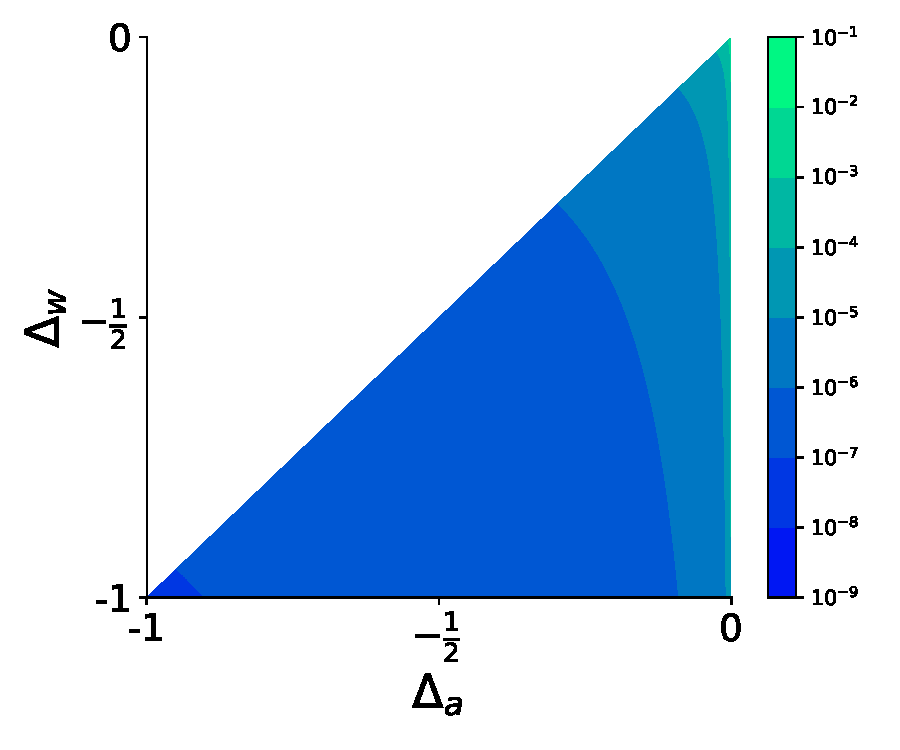
\includegraphics[width=1\textwidth]{Figures/HeatMap_p_est.pdf}
\caption{Contours of the survival probability of an initial population consisting of $10^{3}$ wildtype cells as a function of the
   parameters $\Delta_w=\lambda_w-\mu_w$ and $\Delta_a=\lambda_a-\mu_a$.}
\label{SurvHeatMapPlot}
\end{figure}

%%%%%%%%%%%%%%%%%%%%%%%%%%%%%%%%%%%%%%%%%%
\begin{figure}[!t]
 \vspace*{1\baselineskip}
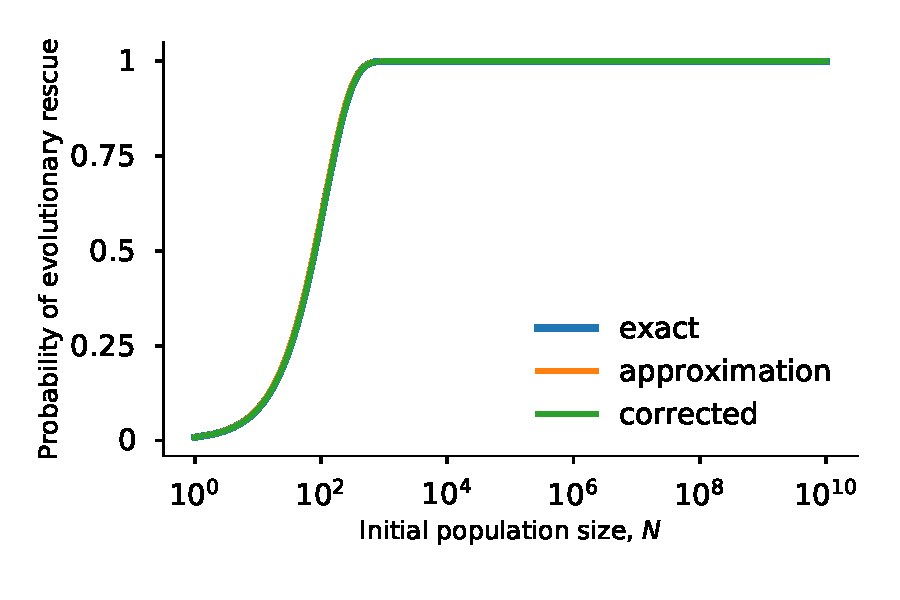
\includegraphics[width=1\textwidth]{Figures/SurvPlotNData.pdf}
\caption{Plot of the probability of survival of a population as a function of the initial population size of wildtype cells. The blue line represents the exact solution \eqref{survprobw}, the orange line line represents the approximation \eqref{aneuploidyresistentfirstapprox}, the green line represents the first order correction \eqref{survprobwapproxcorrected} and the red dots represents stochastic simulations. For the simulations we have chosen the following parameters: $\lambda_w=1-10^{-2}, \lambda_a=1+10^{-2},\lambda_m=1+10^{-1},\mu_w=1,\mu_a=1,\mu_m=1$. The error bars represent $95\%$ confidence interval of the form $p\pm1.96\sqrt{p\left(1-p\right)/n}$ where $p$ is the mean probability of evolutionary rescue and $n$ is the number of simulations.}
\label{SurvPlotNData}
\end{figure}

%%%%%%%%%%%%%%%%%%%%%%%%%%%%%%%%%%%%%%%%%%
\begin{figure}[!t]
 \vspace*{1\baselineskip}
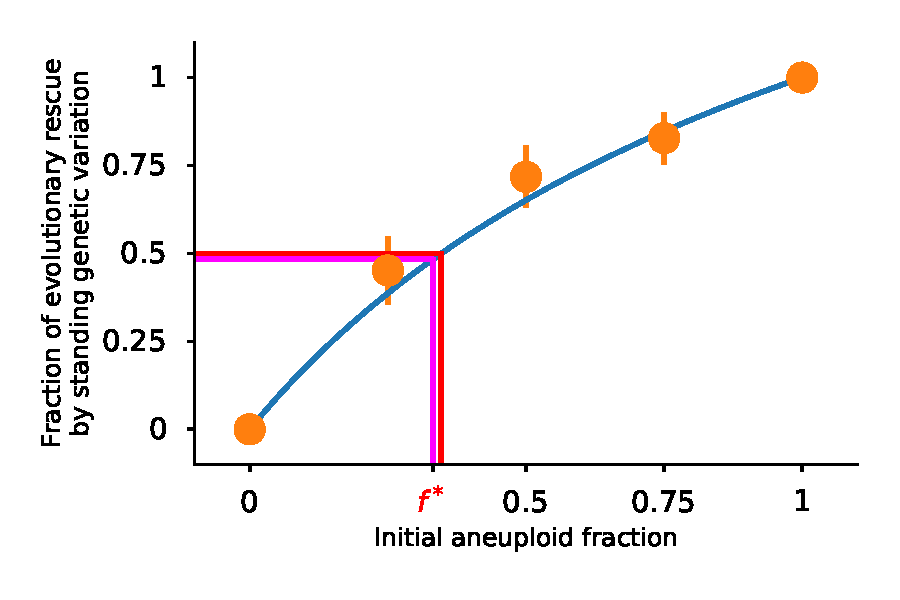
\includegraphics[width=1\textwidth]{Figures/FractionPlot.pdf}
\caption{Plot of the fraction of the cases the population is rescue by standing genetic variation as a function of the fraction of initial cells which are aneuploid. The red vertical line highlights the the value of $f$ for which half the times the population is rescues by aneuploid cells while the pink line is our approximation \eqref{halfeqstandvar}. For this plot we have chosen the following parameters: $N=10^3, \lambda_w=1-10^{-2}, \lambda_a=1-10^{-4},\lambda_m=1+10^{-1},\mu_w=1,\mu_a=1,\mu_m=1$. The error bars represent $95\%$ confidence interval of the form $p\pm1.96\sqrt{p\left(1-p\right)/n}$ where $p$ is the mean probability of evolutionary rescue and $n$ is the number of simulations. The value of $0.332$ highlighted in red is the value of the initial fraction of the population which in aneuploid for which half of the cases of evolutionary rescue is due to initial aneuploid cell population.}
\label{FractionPlot}
\end{figure}


%%%%%%%%%%%%%%%%%%%%%%%%%%%%%%%%%%%%%%%%%%
\section*{Discussion}

%%%%%%%%%%%%%%%%%%%%%%%%%%%%%%%%%%%%%%%%%%

%\section*{References}
\nolinenumbers
%\bibliographystyle{agsm}
%\bibliographystyle{apalike}
%\bibliographystyle{unsrtnat}
\bibliographystyle{unsrt}
\bibliography{evo2022}
\pagebreak

%%%%%%%%%%%%%%%%%%%%%%%%%%%%%%%%%%%%%%%%%%
%\appendix
\begin{appendices}
\renewcommand{\theequation}{\thesection\arabic{equation}}
\counterwithin*{equation}{section}


%%%%%%%%%%%%%%%%%%%%%%%%%%%%%%%%%%%%%%%%%%
%\section*{Gillespie algorithm}
%\begin{subequations}
%\begin{flalign}
%(+1,0,0)&:\quad \lambda_ww_t,\\
%(-1,0,0)&:\quad \mu_ww_t,\\
%(-1,+1,0)&:\quad uw_t,\\
%(-1,0,+1)&:\quad vw_t,\\
%(0,+1,0)&:\quad \lambda_aa_t,\\
%(0,-1,0)&:\quad \mu_aa_t,\\
%(0,-1,+1)&:\quad va_t,\\
%(0,0,+1)&:\quad \lambda_am_t,\\
%(0,0,-1)&:\quad \mu_am_t.
%\end{flalign}
%\end{subequations}

%%%%%%%%%%%%%%%%%%%%%%%%%%%%%%%%%%%%%%%%%%
\section{Survival probability of a mutant lineage}\label{AppendixSurvLin}
The infinitesimal transition probabilities for the simple birth and death process:
\begin{align*}
p_{i+j,i}\left(\Delta t\right)=\left\{
  \begin{array}{@{}ll@{}}
  \mu i\Delta t+o\left(\Delta t\right),\quad j=-1 \\
  \lambda i\Delta t+o\left(\Delta t\right),\quad j=1 \\
    1-\left(\lambda+\mu\right) i\Delta t+o\left(\Delta t\right),\quad j=0 \\
   o\left(\Delta t\right),\quad j\neq-1,0,1.
  \end{array}\right.
\end{align*}
The forward Kolmogorov differential equations are:
\begin{subequations}
\label{KolmeqSurv}
\begin{flalign}
\frac{dp_i\left(t\right)}{dt}&=\lambda\left(i-1\right)p_{i-1}\left(t\right)+\mu\left(i+1\right)p_{i+1}\left(t\right)-\left(\lambda+\mu\right)ip_i\left(t\right),\\
\frac{dp_0\left(t\right)}{dt}&=\mu p_1\left(t\right),
\end{flalign}
\end{subequations}
for $i=1,2,\dots$ with initial conditions $p_i\left(0\right)=\delta_{iN}$.

The probability generating function is defined as:
\begin{equation*}
\mathcal{P}\left(z,t\right)=\sum_{i=0}^\infty p_i\left(t\right)z^i
\end{equation*}
which we obtain by multiplying \eqref{KolmeqSurv} by $z^i$ and summing over $i$:
\begin{align*}
\mathcal{P}\left(z,t\right)=\left\{
  \begin{array}{@{}ll@{}}
  \left(\frac{\e^{t\left(\mu-\lambda\right)}\left(\lambda z-\mu\right)-\mu\left(z-1\right)}{\e^{t\left(\mu-\lambda\right)}\left(\lambda z-\mu\right)-\lambda\left(z-1\right)}\right)^N,\quad \text{if }\lambda\neq\mu, \\
  \left(\frac{1-\left(\lambda t-1\right)\left(z-1\right)}{1-\lambda t\left(z-1\right)}\right)^N,\quad \text{if }\lambda=\mu.
  \end{array}\right.
\end{align*}
The probability $p_i$ can be obtained from the probability generating function as:
\begin{equation*}
p_i\left(t\right)=\left.\frac{1}{i!}\frac{\partial^i\mathcal{P}}{\partial z^i}\right|_{z=0},
\end{equation*}
and the probability of extinction is given by:
\begin{align*}
p_0\left(t\right)=\left\{
  \begin{array}{@{}ll@{}}
  \left(\frac{\mu-\mu\e^{\left(\mu-\lambda\right)t}}{\lambda-\mu\e^{\left(\mu-\lambda\right)t}}\right)^N,\quad \text{if }\lambda\neq\mu, \\
  \left(\frac{\lambda t}{1+\lambda t}\right)^N,\quad \text{if }\lambda=\mu.
  \end{array}\right.
\end{align*}
When $t\rightarrow\infty$ the extinction probability has the following expression:
\begin{align*}
p_0\left(\infty\right)=\lim_{t\rightarrow\infty}p_0\left(t\right)=\left\{
  \begin{array}{@{}ll@{}}
  1,\quad \text{if }\lambda\leq\mu, \\
  \left(\frac{\mu}{\lambda}\right)^N,\quad \text{if }\lambda>\mu.
  \end{array}\right.
\end{align*}
%%%%%%%%%%%%%%%%%%%%%%%%%%%%%%%%%%%%%%%%%%
\section*{Mean time}
%%%%%%%%%%%%%%%%%%%%%%%%%%%%%%%%%%%%%%%%%%
We define the following events
\begin{align*}
\text{EvR}&=\text{``evolutionary rescue occurs''},\\
\text{EvRA}&=\text{``evolutionary rescue occurs through aneuploidy''},\\
\text{EvRM}&=\text{``evolutionary rescue occurs through mutation''}.
\end{align*}
As a result, the mean time to appearence of the first mutant cell which rescues the population given evolutionary rescue can be expanded as:
\begin{align*}
\mathbb{E}\left[\tau|\text{EvR}\right]&=\mathbb{E}\left[\tau|\text{EvR},\text{EvRA}\cap\text{EvRM}^{C}\right]p\left(\text{EvRA}\cap\text{EvRM}^{C}|\text{EvR}\right)\\
&+\mathbb{E}\left[\tau|\text{EvR},\text{EvRM}\cap\text{EvRA}^{C}\right]p\left(\text{EvRM}\cap\text{EvRA}^{C}|\text{EvR}\right)\\
&+\mathbb{E}\left[\tau|\text{EvR},\text{EvRM}\cap\text{EvRA}\right]p\left(\text{EvRM}\cap\text{EvRA}|\text{EvR}\right).
\end{align*}
The joint probabilities in the previous lines can be written as:
\begin{align*}
p\left(\text{EvRA}\cap\text{EvRM}^{C}|\text{EvR}\right)&=\frac{p\left(\text{EvRA}\cap\text{EvRM}^{C}\right)}{p\left(\text{EvR}\right)}
\approx\frac{p\left(\text{EvRA}\right)\left[1-p\left(\text{EvRM}\right)\right]}{p\left(\text{EvR}\right)},\\
p\left(\text{EvRM}\cap\text{EvRA}^{C}|\text{EvR}\right)&=\frac{p\left(\text{EvRM}\cap\text{EvRA}^{C}\right)}{p\left(\text{EvR}\right)}
\approx\frac{p\left(\text{EvRM}\right)\left[1-p\left(\text{EvRA}\right)\right]}{p\left(\text{EvR}\right)},\\
p\left(\text{EvRM}\cap\text{EvRA}|\text{EvR}\right)&=\frac{p\left(\text{EvRM}\cap\text{EvRA}\right)}{p\left(\text{EvR}\right)}\approx\frac{p\left(\text{EvRM}\right)p\left(\text{EvRA}\right)}{p\left(\text{EvR}\right)}\ll1.
\end{align*}
As a result, we have:
\begin{align*}
\mathbb{E}\left[\tau|\text{EvR}\right]&\approx\mathbb{E}\left[\tau|\text{EvR},\text{EvRA}\cap\text{EvRM}^{C}\right]p\left(\text{EvRA}\cap\text{EvRM}^{C}|\text{EvR}\right)\\
&+\mathbb{E}\left[\tau|\text{EvR},\text{EvRM}\cap\text{EvRA}^{C}\right]p\left(\text{EvRM}\cap\text{EvRA}^{C}|\text{EvR}\right).
\end{align*}
%%%
%%%%%%%%%%%%%%%%%%%%%%%%%%%%%%%%%%%%%%%%%%
\section*{Diffusion approximation}\label{AppendixDiffApprox}
%%%%%%%%%%%%%%%%%%%%%%%%%%%%%%%%%%%%%%%%%%
\begin{equation}
r=\lim_{\Delta t\rightarrow0}\frac{\mathbb{E}\left(\Delta n_t|n_t\right)}{\Delta_t n_t}
\end{equation}
\begin{equation}
\sigma=\lim_{\Delta t\rightarrow0}\frac{\mathbb{V}ar\left(\Delta n_t|n_t\right)}{\Delta_t n_t}
\end{equation}
\begin{align}
\lambda_1=v\pi_f\frac{w_0}{|r_w|}
\end{align}
where
\begin{align}
\bar{\pi}_f=\int_{0}^\infty\int_{0}^\infty \left(1-\e^{\frac{-2r}{\sigma}}\right) f_r\left(r,\sigma\right)\d r\d\sigma
\end{align}
Let $f\left(r,\sigma\right)=\delta\left(r-r_m\right)\delta\left(\sigma-\sigma_m\right)$ then:
\begin{align}
\bar{\pi}_f=1-\e^{\frac{-2r_m}{\sigma_m}}
\end{align}
\begin{align}
\lambda_1=v\left(1-\e^{\frac{-2r_m}{\sigma_m}}\right)\frac{N_0}{|\Delta_w|}
\end{align}
\begin{align}
\lambda_2&=\frac{uw_0}{|r_w|}\int_{0}^\infty\int_{0}^\infty \left(1-\pi_f\left(r,q\right)\right) f_r\left(r,\sigma\right) p_1^*\left(r,\sigma\right)\d r\d\sigma\\
&=\frac{uw_0}{|\Delta_w|}p_1^*\left(r_a,\sigma_a\right)\\
&=\frac{uw_0}{|\Delta_w|}\left[1-\exp\left(-\frac{|\Delta_a|}{|\lambda_a+\mu_a|}\right)\left(\sqrt{1+\frac{2\sigma_a^2}{r_a^2}u^*}-1\right)\right]
\end{align}
where
\begin{equation}
u^*=v\left(1-\e^{\frac{-2r_m}{\sigma_m}}\right)
\end{equation}
The number of rescue mutations has a Poisson distribution with rate $\lambda_1+\lambda_2$. As a result, the probability of evolutionary rescue is given by:
\begin{equation}
p_{est}=1-\e^{-\left(\lambda_1+\lambda_2\right)}
\end{equation}

\end{appendices}

\newpage
\section*{Supplementary Figures}
\beginsupplement % https://support.authorea.com/en-us/article/how-to-create-an-appendix-section-or-supplementary-information-1g25i5a/

%%%%%%%%%%%%%%%%%%%%%%%%%%%%%%%%%%%%%%%%%%
\end{document}